\documentclass[hyperref={pdfpagelabels=false}]{beamer}
\usepackage{listings}
\usepackage{xcolor}


\definecolor{codegreen}{rgb}{0,0.6,0}
\definecolor{codegray}{rgb}{0.5,0.5,0.5}
\definecolor{codepurple}{rgb}{0.58,0,0.82}
\definecolor{backcolour}{rgb}{0.95,0.95,0.92}

\lstdefinestyle{mystyle}{
    backgroundcolor=\color{backcolour},   
    commentstyle=\color{codegreen},
    keywordstyle=\color{magenta},
    numberstyle=\tiny\color{codegray},
    stringstyle=\color{codepurple},
    basicstyle=\ttfamily\footnotesize,
    breakatwhitespace=false,         
    breaklines=true,                 
    captionpos=b,                    
    keepspaces=true,                 
    numbers=left,                    
    numbersep=5pt,                  
    showspaces=false,                
    showstringspaces=false,
    showtabs=false,                  
    tabsize=2
}

\lstset{style=mystyle}
% Contact information: 
%   Jorge M. Cruz-Duarte (jorge.cruz@tec.mx)
%   Nov. 29, 2019

\usepackage{lmodern, ragged2e, CJKutf8, booktabs, subfigure, graphicx, algorithm, algorithmicx, algpseudocode, amsmath, amssymb, amsthm, amsfonts, mathtools, multirow}
\usepackage[style=phys]{biblatex}
\addbibresource{bibliography.bib}
\renewcommand{\footnotesize}{\tiny}
\makeatletter
\@newctr{footnote}[page]
\makeatother
\usetheme{CambridgeUS}
\renewcommand{\raggedright}{\leftskip=0pt \rightskip=0pt plus 0cm}



\definecolor{TEC blue}{RGB}{0, 32, 159}
\newcommand{\hl}[1]{{\textcolor{TEC blue}{#1}}}

% Theme setup
\titlegraphic{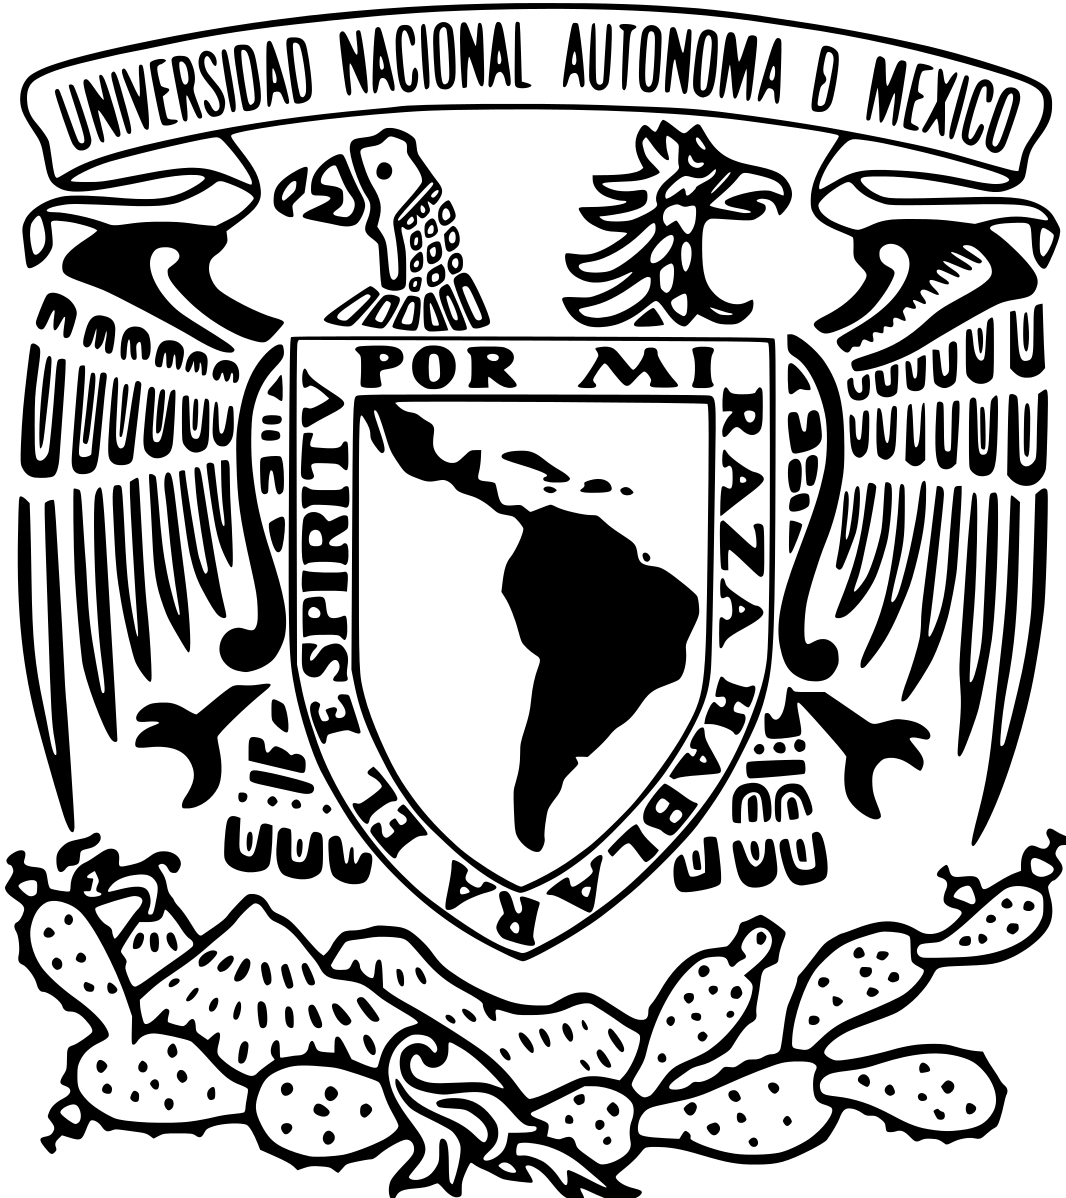
\includegraphics[scale=0.07]{Figures/logounam.png}}

% \makeatletter
\setbeamertemplate{headline}{%
\leavevmode%
  \hbox{%
    \begin{beamercolorbox}[wd=\paperwidth,ht=2.5ex,dp=1.125ex]{palette quaternary}%
    \insertsectionnavigationhorizontal{\paperwidth}{}{\hskip0pt plus1filll}
    \end{beamercolorbox}%
  }
}
\setbeamertemplate{footline}{\hspace*{2ex} \insertshortauthor \hfill \textcolor{TEC blue}{\insertshorttitle} \hfill \textbf{\insertframenumber{}} / \inserttotalframenumber \hspace*{2ex}}

\setbeamercolor{item projected}{bg=TEC blue}
\setbeamertemplate{enumerate items}[default]
\setbeamercolor*{enumerate item}{fg=TEC blue}

\setbeamertemplate{navigation symbols}{} 
% \setbeamertemplate{footline}[\insertshorttitle frame number]
\setbeamertemplate{bibliography item}[text]
\setbeamertemplate{theorems}[numbered]

\setbeamerfont{title}{series = \bfseries, parent = structure}
\setbeamerfont{frametitle}{series = \bfseries, parent = structure}
\setbeamerfont{headline}{series = \bfseries, size = \tiny, parent = structure}

\setbeamercolor{title}{fg = white, bg = TEC blue}
\setbeamercolor{frametitle}{fg = white, bg = TEC blue}
\setbeamercolor{structure}{fg = TEC blue}
\setbeamercolor{section in head/foot}{fg = black, bg = TEC blue!40}
\setbeamercolor{subsection in head/foot}{fg = black, bg = TEC blue!20}

\setbeamercolor{block title}{use=structure,fg=white,bg=structure.fg!75!black}
\setbeamercolor{block body}{parent=normal text,use=block title,bg=TEC blue!20} %block title.bg!10!bg}
\makeatletter
\def\th@mystyle{%
    \normalfont % body font
    \setbeamercolor{block title example}{bg=orange,fg=white}
    \setbeamercolor{block body example}{bg=orange!20,fg=black}
    \def\inserttheoremblockenv{exampleblock}
  }
\makeatother
\theoremstyle{mystyle}
\newtheorem*{remark}{Remark}

\usepackage{tikz}
\setbeamertemplate{background}{\tikz[overlay,remember picture]\node[opacity=0.05]at (current page.center){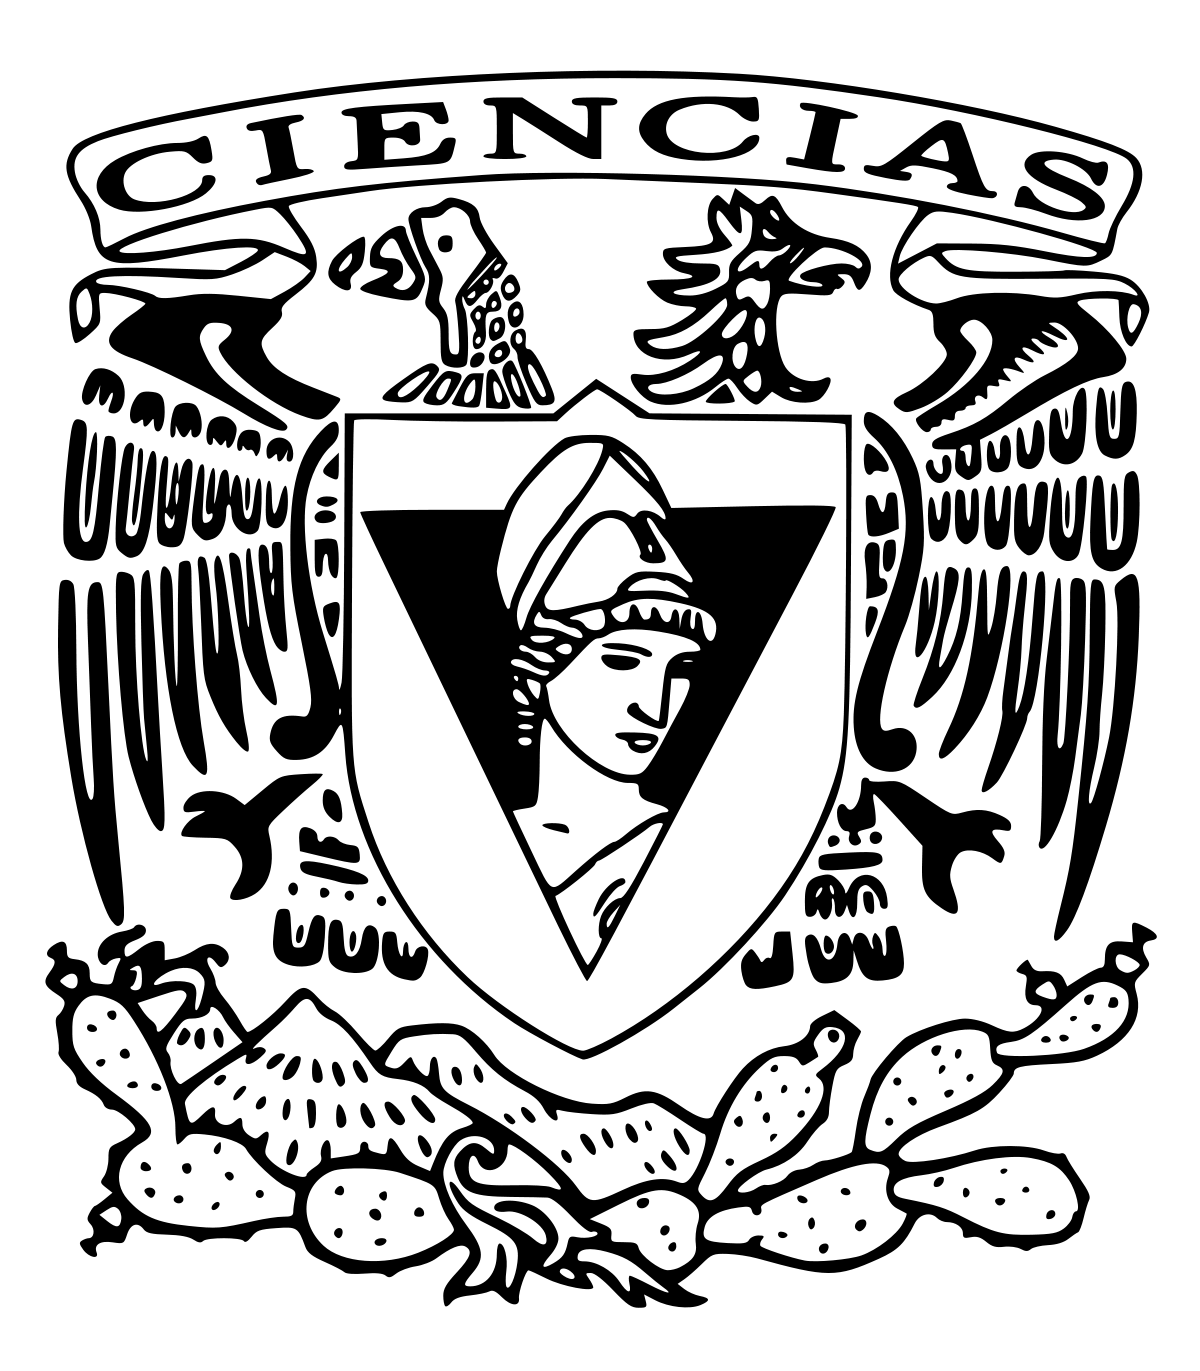
\includegraphics[width=6cm]{Figures/logociencias.png}};}


\newcommand{\maketitleandtoc}{%
{%
    \setbeamertemplate{headline}{}%
    \setbeamertemplate{footline}{}%
    \begin{frame}[noframenumbering]%
        \titlepage%
    \end{frame}%
    \begin{frame}[noframenumbering]%
        \frametitle{Contenido}%
        \tableofcontents%
    \end{frame}%
}}

\newcommand{\noheadfoot}[1]{%
    {%
        \setbeamertemplate{headline}{}%
        \setbeamertemplate{footline}{}%
        {#1}
    }
}

\title{Chaos and the Lorenz System}  
\author[Facultad de Ciencias, UNAM]{Miguel Ángel Sánchez Cortés} 
\institute{Facultad de Ciencias, UNAM} 
\date{\today}

\begin{document}

\maketitleandtoc

\section{Introduction}
\begin{frame}{The Lorenz Equations}\justifying

In 1960, Edward Lorenz proposed an innovative mathematical model intended to predict the weather. The crucial ingredient for this model was \textbf{convection}. 

\vspace{10pt}

\begin{figure}
        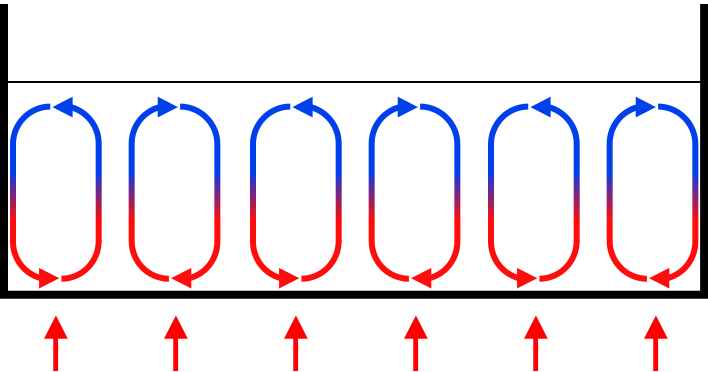
\includegraphics[width=0.6\linewidth]{conveccion.png}\\ \vspace{0.5cm}
    \end{figure}

\vspace{-15pt}
In this project we pretend to solve computationally the Lorenz Equations and analyze their consequences. 

\end{frame}
\begin{frame}{Las ecuaciones de Lorenz}

To be able to solve the governing equations for convection using the computational power of his time, Lorenz simplified his equations and reduced them to the following system:

\vspace{10pt}
\begin{block}{Lorenz Equations}
\begin{equation*}
\dot{x}=\sigma(y-x) \hspace{5pt} \text{;} \quad \dot{y}=x(\rho-z)-y \quad \text{;} \quad \dot{z}=xy-\beta z
\end{equation*}
\end{block}

\vspace{10pt}

where $\rho>0$ quantifies the difference in temperature $\Delta T$, $\beta>0$ quantifies the relative height of the layer of fluid and $\sigma>0$ quantifies the loss of energy due to viscosity and thermal conduction.

\end{frame}
\begin{frame}{Las ecuaciones de Lorenz}

Before solving this equations is important to notice that we can find the fixed point of the systems. This points are:

\begin{block}{Fixed points of the Lorenz System}
\begin{equation*}
 \Vec{x*}=(0,0,0) \quad \text{,} \quad C^{\pm}=(\pm\sqrt{\beta(\rho-1)},\pm \sqrt{\beta(\rho-1)},\rho-1) 
 \end{equation*}
\end{block}
\vspace{-15pt}
\begin{figure}
        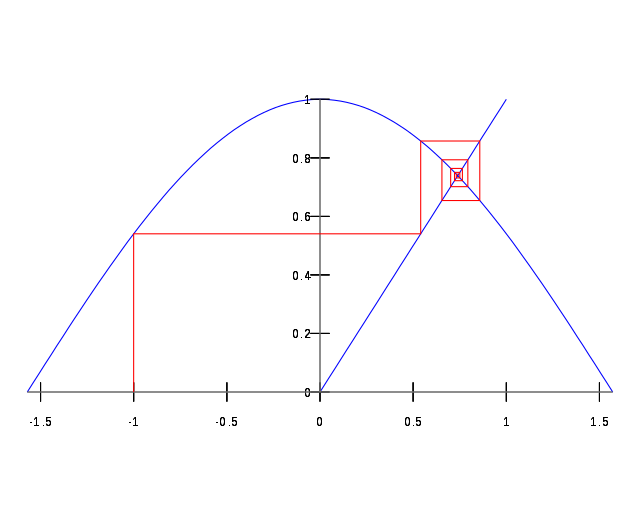
\includegraphics[width=0.55\linewidth]{Figures/fixed.png}\\ 
    \end{figure}


\end{frame}

\section{Desarrollo} 
\begin{frame}{The 4th Order Runge-Kutta method} 

To solve the Lorenz system, we used the 4th order Runge-Kutta method programmed in Fortran. This method takes a system of 3 equations:

\begin{block}{ODE system}
\begin{equation*}
\frac{dx}{dt}=f(x,y,z) \quad \text{,} \quad \frac{dy}{dt}=g(x,y,z) \quad \text{,} \quad \frac{dz}{dt}=u(x,y,z)
\end{equation*}
\end{block}

\vspace{10pt}

with $x(t_{0})=x_{0}$, $y(t_{0})=y_{0}$ and $z(t_{0})=z_{0}$, and solves it iteratively advancing the solution of $x$ $y$ y $z$ to $t_{i}=t_{i-1}+h$ with $h=(b-a)/n$ so that the solutions are:

\begin{block}{The 4th Order Runge-Kutta method}
\begin{equation*}
x_{i+1}=x_{i}+(K_{0}+2K_{1}+2K_{2}+K_{3})/6 \quad \text{,} \quad y_{i+1}=y_{i}+(L_{0}+2L_{1}+2L_{2}+L_{3})/6 
\end{equation*}
\end{block}




\end{frame}
\begin{frame}{The 4th Order Runge-Kutta method}

\begin{block}{The 4th Order Runge-Kutta method}
\begin{equation*}
z_{i+1}=z_{i}+(M_{0}+2M_{1}+2M_{2}+M_{3})/6 
\end{equation*}
\end{block}
\vspace{10pt}

with the coefficients given by:

\begin{equation*}
K_{0}=hf(x_{i},y_{i},z_{i}) \quad \text{,} \quad L_{0}=hg(x_{i},y_{i},z_{i}) \quad \text{y} \quad M_{0}=hu(x_{i},y_{i},z_{i})
\end{equation*}

\begin{equation*}
K_{n}=hf(x_{i}+\frac{1}{2}K_{n-1},y_{i}+\frac{1}{2}L_{n-1},z_{i}+\frac{1}{2}M_{n-1}) \quad \forall n \in {1,2}
\end{equation*}
\begin{equation*}
L_{n}=hg(x_{i}+\frac{1}{2}K_{n-1},y_{i}+\frac{1}{2}L_{n-1},z_{i}+\frac{1}{2}M_{n-1}) \quad \forall n \in {1,2}
\end{equation*}

\begin{equation*}
M_{n}=hu(x_{i}+\frac{1}{2}K_{n-1},y_{i}+\frac{1}{2}L_{n-1},z_{i}+\frac{1}{2}M_{n-1}) \quad \forall n \in {1,2}
\end{equation*}



    
\end{frame}

\begin{frame}{The 4th Order Runge-Kutta method}

\begin{equation*}
K_{3}=hf(x_{i}+K_{2},y_{i}+L_{2},z_{i}+M_{2}) \quad \text{;} \quad L_{3}=hg(x_{i}+K_{2},y_{i}+L_{2},z_{i}+M_{2})
\end{equation*}



\begin{equation*}
M_{3}=hu(x_{i}+K_{2},y_{i}+L_{2},z_{i}+M_{2})
\end{equation*}

\begin{figure}
        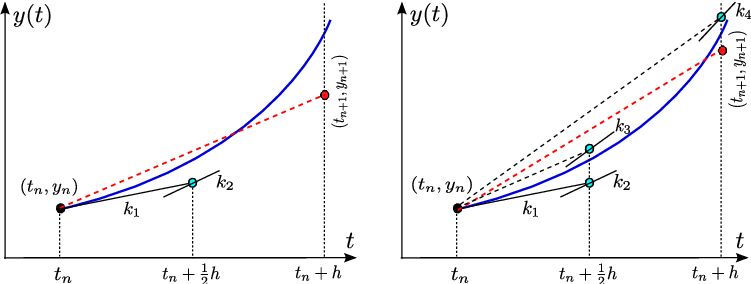
\includegraphics[width=0.8\linewidth]{Figures/4thorder.png}\\ \vspace{10pt}
    \end{figure}

\end{frame}



\section{Resultados}

\begin{frame}{Global stability, $0<\rho<1$}

Mathematically, near the origin, the solution of the system remains stable and tends to zero. Mathematically,  $z(t)\rightarrow0$ for $t\rightarrow \infty$. If $\rho<1$, the trajectories in $x$ and $y$ approximate the origin as well, thus we conclude that the origin is \textbf{globally stable}.



\begin{block}{Two solutions}
$\sigma=10$, $\beta=8/3$ y $\rho=0.9$ for $\Vec{x_{0}}=(-10,10,5)$ and for $\Vec{x_{0}}=(10,3,-4)$.
\end{block}

\begin{figure}

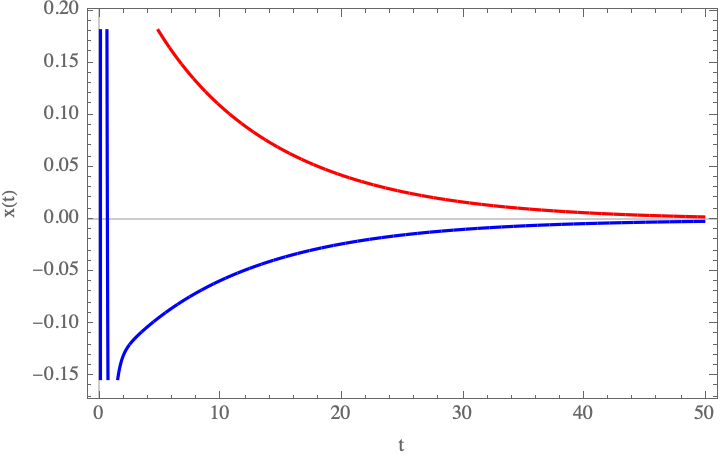
\includegraphics[width=0.6\linewidth]{Figures/seriesdetiempo.png}

\end{figure}

    
\end{frame}

\begin{frame}{Global stability, $0<\rho<1$}

\begin{figure}

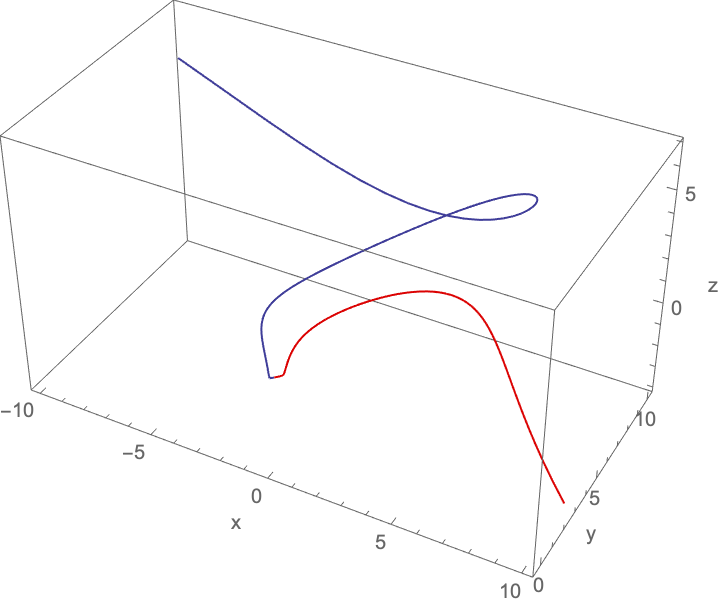
\includegraphics[width=0.75\linewidth]{Figures/atractores.png}

\end{figure}

\end{frame}

\begin{frame}{Stability in $C^{+}$ y $C^{-}$ for $1<\rho<\rho_{c}$}

Mathematically if $\rho>1$, the trajectories in $x$ and $y$ are on a cycle and the motion around $C^{+}$ and $C^{-}$ is stable for:
\begin{equation*}
1<\rho<\rho_{c}=\frac{\sigma(\sigma + \beta + 3)}{\sigma -\beta -1} \quad \text{assuming that:} \hspace{5pt} \sigma - \beta -1 >0
\end{equation*}

\vspace{-5pt}
\begin{block}{One solution:}
\centering
$\sigma=10$, $\beta=8/3$ and $\rho=14$ for $\Vec{x_{0}}=(0,1,0)$.
\end{block}

\begin{figure}

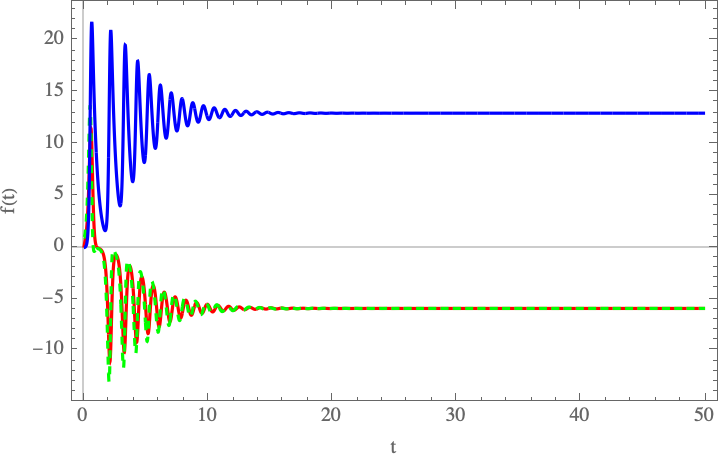
\includegraphics[width=0.6\linewidth]{Figures/estabilidad.png}

\end{figure}

\end{frame}

\begin{frame}{Stability in $C^{+}$ y $C^{-}$ for $1<\rho<\rho_{c}$}

\begin{figure}

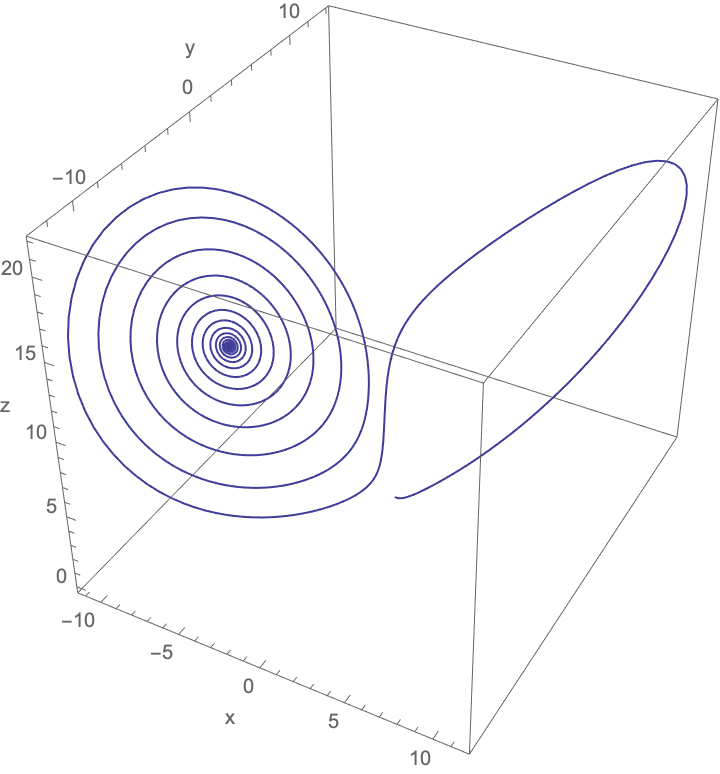
\includegraphics[width=0.6\linewidth]{Figures/espiral.png}

\end{figure}

\end{frame}

\begin{frame}{Chaos for $\rho>\rho_{c}$}

In this case, the trajectories are constantly repelled by the $C^{+}$ and $C^{+}$ points like in a pinball machine and don't converge to a stable point.
 
\begin{block}{The Lorenz Attractor}
\centering
$\sigma=10$, $\beta=8/3$ and $\rho=28$ for $\Vec{x_{0}}=(0,1,0)$.
\end{block}

\begin{figure}

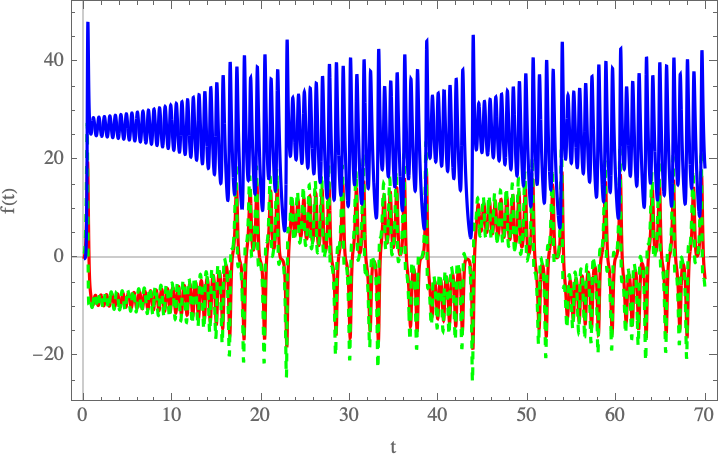
\includegraphics[width=0.65\linewidth]{Figures/seriedetiempo.png}

\end{figure}

\end{frame}

\begin{frame}{Chaos for $\rho>\rho_{c}$}

\begin{figure}

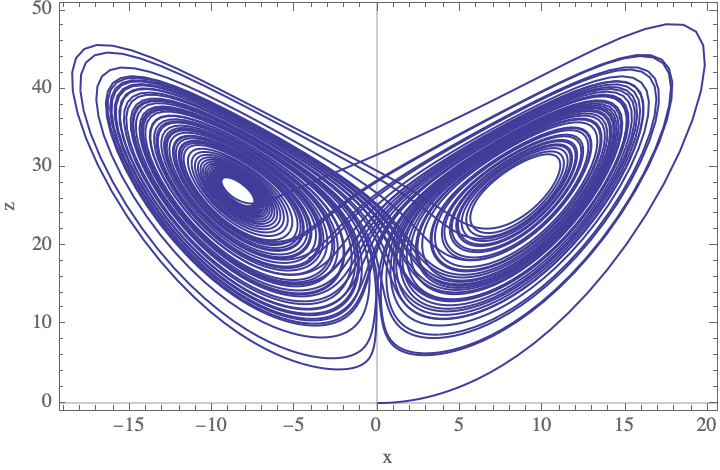
\includegraphics[width=0.9\linewidth]{Figures/atractor2d.png}

\end{figure}

\end{frame}

\begin{frame}{Chaos for $\rho>\rho_{c}$}

\begin{figure}

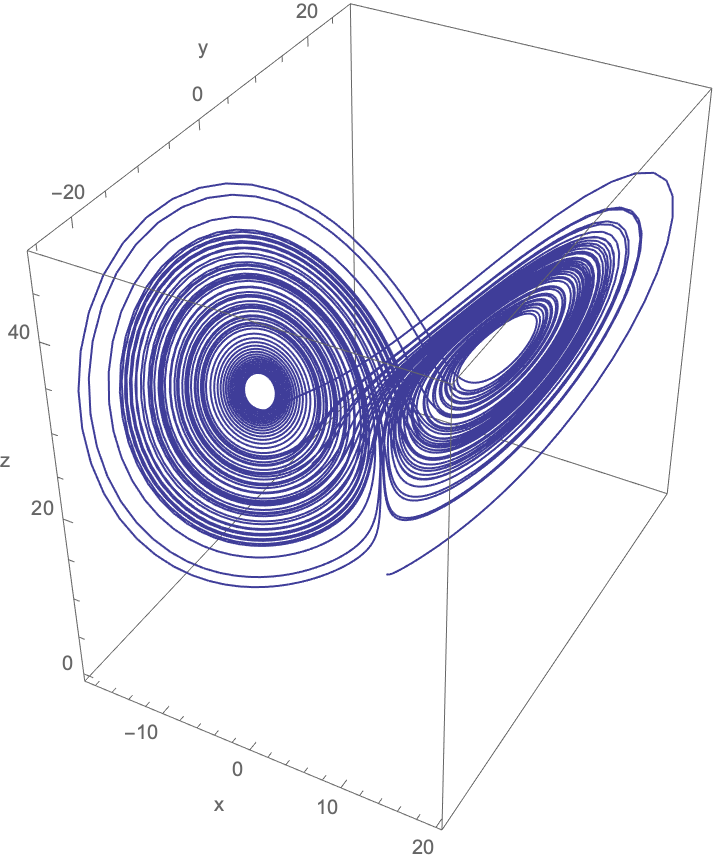
\includegraphics[width=0.55\linewidth]{Figures/atractor3d.png}

\end{figure}

\end{frame}

\begin{frame}{The butterfly effect}

This system exhibits \textbf{extreme sensibility to initial conditions}. At first, the trajectories of very similar initial conditions, for example separated by $\delta_{0}=1\times 10^{-12}$, are very similar. Nevertheless, when time goes by, the trajectories diverge completely.

\begin{block}{Two solutions}
$\sigma=10$, $\beta=8/3$ and $\rho=28$ for $\Vec{x_{0}}=(0,1,0)$ y para $\Vec{x_{0}}=(\delta_{0},1+\delta_{0},\delta_{0})$.
\end{block}


\begin{figure}

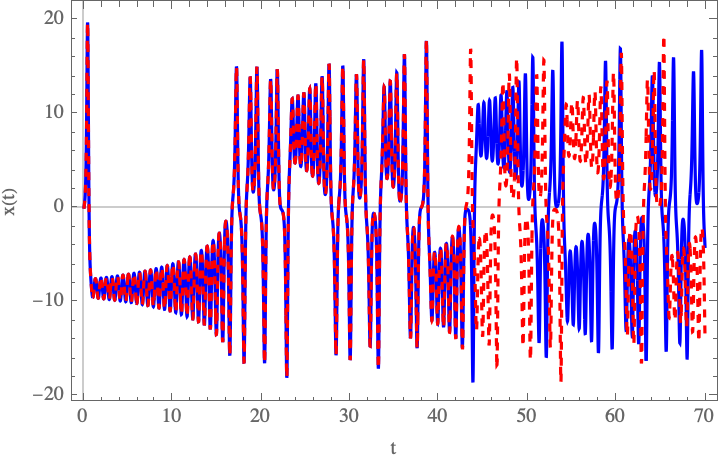
\includegraphics[width=0.6\linewidth]{Figures/comparacionx.png}

\end{figure}

\end{frame}

\begin{frame}{The butterfly effect}

\begin{figure}

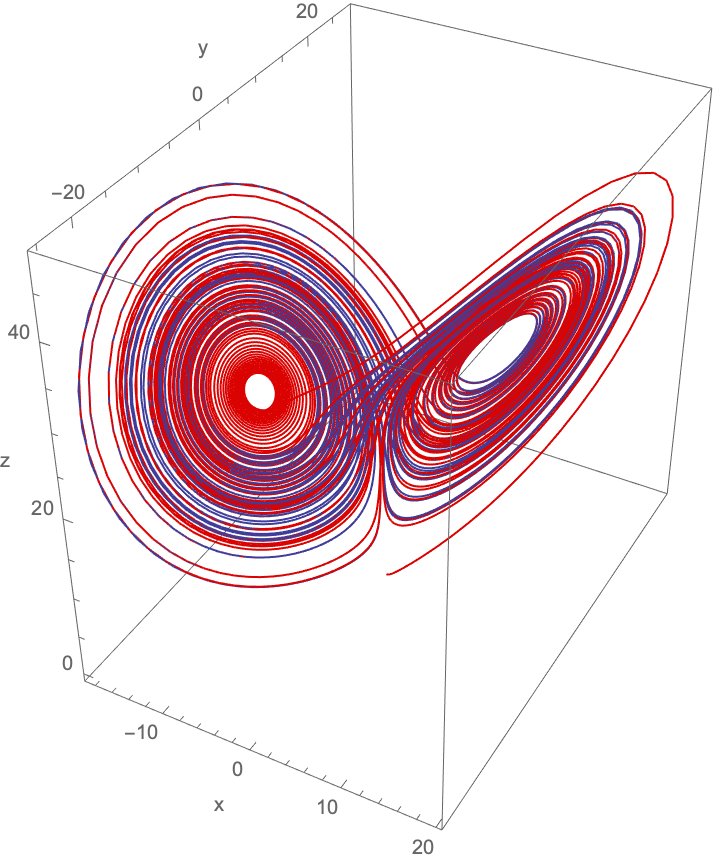
\includegraphics[width=0.55\linewidth]{Figures/comparacionatractor3d.png}

\end{figure}

\end{frame}

\begin{frame}{The butterfly effect}
Let's suppose we have a point $x(t)$ in the attractor at time $t$ and we take another point $x(t)+\delta (t)$ such that initially $\delta(0)= \lVert \delta_{0} \rVert \ll 1$. If we plot $\ln(\lVert \delta(t)\rVert)$ vs $t$:

\begin{figure}

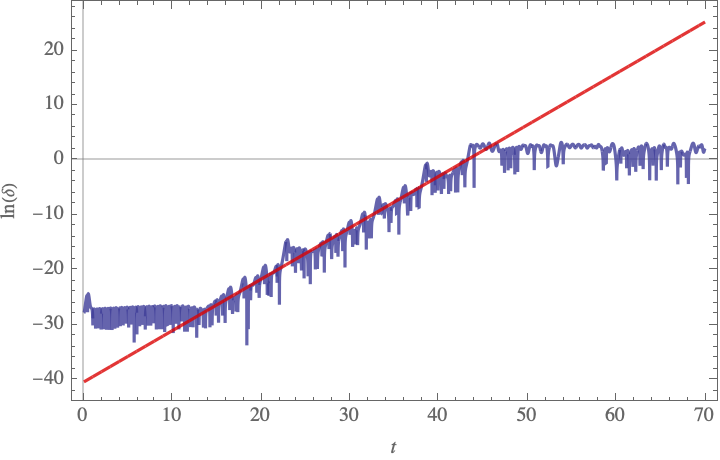
\includegraphics[width=0.6\linewidth]{Figures/ajuste.png}

\end{figure}
\vspace{-10pt}

We find a graph similar to a linear fit with positive slope $\lambda \approx 0.93$. This means that $\lVert \delta(t) \rVert \sim \lVert \delta_{0} \rVert e^{\lambda t}$. This $\lambda$ is known as the \textbf{Lyapunov coefficient}.

\end{frame}

\begin{frame}{The Lorenz map}
In 1963 Lorenz found a way to analyze the dynamics of his strange attractor. The idea was that the local maxima of $z(t)$, $z_{n}$ should predict the $z_{n+1}$. If we plot $z_{n+1}$ vs $z_{n}$:

\begin{figure}

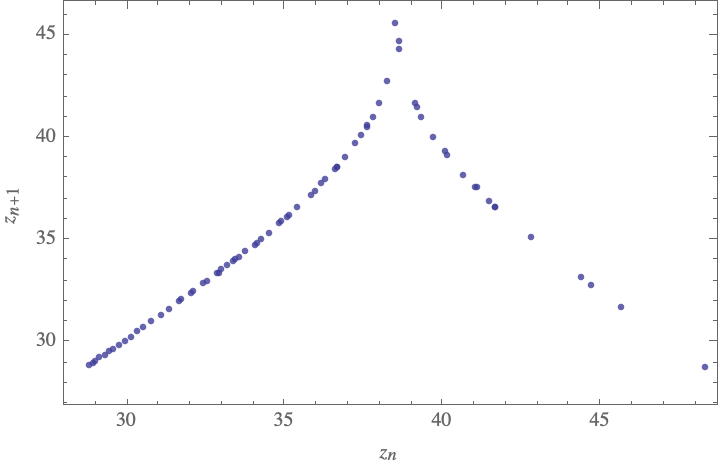
\includegraphics[width=0.6\linewidth]{Figures/mapeo.png}

\end{figure}

\vspace{-10pt}

We find an almost smooth function $z_{n+1}=f(z_{n})$ that is known as the \textbf{Lorenz map}.
\end{frame}

\begin{frame}{The bifurcation diagram}
$\rho$ plays a crucial part in the trajectory of the system. When we change this parameter we can find infinite cases: limit cycles, intermittent chaos or strange attractors, the possibilities are endless.

\begin{figure}

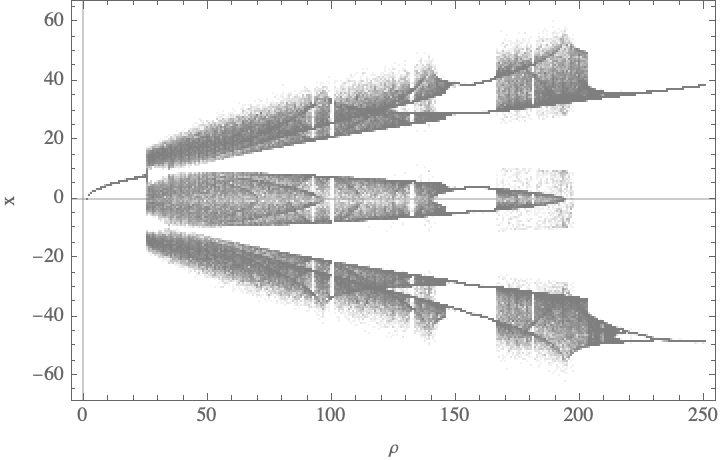
\includegraphics[width=0.8\linewidth]{Figures/x.png}

\end{figure}


\end{frame}

\begin{frame}{The bifurcation diagram}
 

\begin{figure}

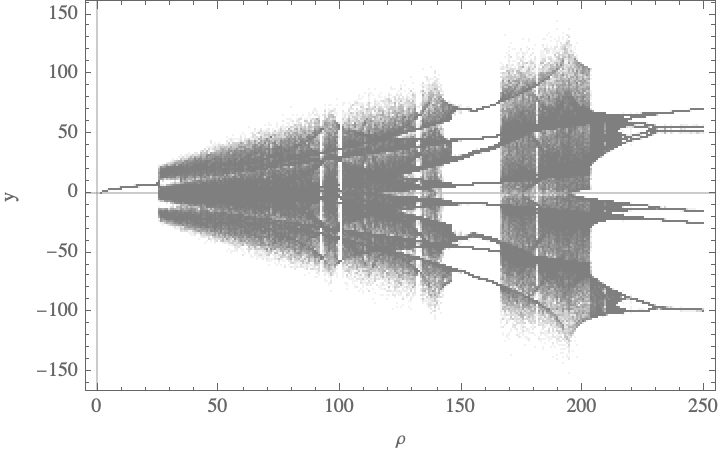
\includegraphics[width=\linewidth]{Figures/y.png}

\end{figure}


\end{frame}

\begin{frame}{The bifurcation diagram}
 

\begin{figure}

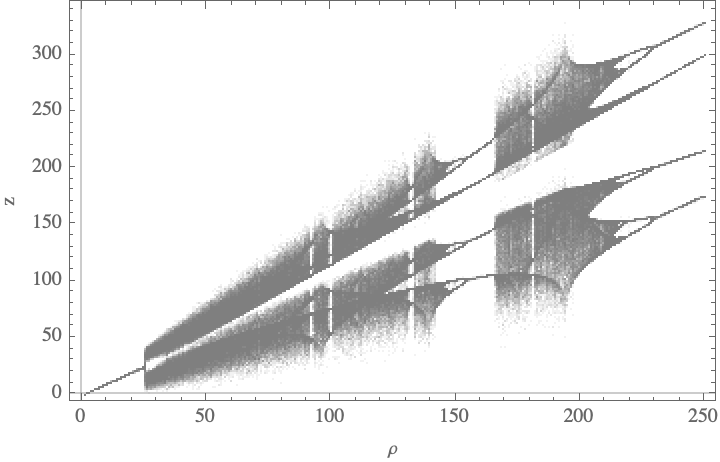
\includegraphics[width=\linewidth]{Figures/z.png}

\end{figure}


\end{frame}


\section{References}

\begin{frame}{References}
\begin{thebibliography}{9}
\bibitem{strogatz} 
Steven H. Strogatz
\textit{Nonlinear Dynamics and Chaos}. 
Perseus Books, Reading, Massachusetts, 1994.

\bibitem{gleick} 
James Gleick
\textit{Chaos: making a new science}. 
Penguin Books, 2008.

\bibitem{boeing} 
Boeing G. 
\textit{Visual Analysis of Nonlinear Dynamical Systems: Chaos, Fractals, Self-Similarity and the Limits of Prediction}. 
Systems, 4(4),37, 2016.

\bibitem{difference} 
Song W., Liang J. 
\textit{Difference equation of Lorenz system}. 
International Journal of Pure and Applied Mathematics, 83(1),101-110, 2013.


\end{thebibliography}

    
\end{frame}


\noheadfoot{
\begin{frame}[noframenumbering]
\begin{minipage}[c]{0.3\linewidth}
\begin{flushright}
    \Large{
    \par \hl{!`Gracias!}
    \begin{CJK*}{UTF8}{gbsn}
    \par 谢谢!
    \par ありがとう!
    \end{CJK*}
    \par Thanks!
    \par Grazie!
    \par Merci!
    \par Mul\c{t}mesc!}
\end{flushright}
\end{minipage}\hspace{0.1cm}%
\begin{minipage}[c]{0.45\linewidth}
    \begin{flushleft}
        
\includegraphics[width=0.8\linewidth]{Figures/newton.png}
    \end{flushleft}
\end{minipage}%
\begin{flushright}
    \line(1,0){135}\\
    \textbf{Contact:}\\
    \hl{Miguel Ángel Sánchez Cortés}\\
    E-mail: \texttt{miguel.sanchezcortes@ciencias.unam.mx}\\
    \textit{Alumni}\\
    Facultad de Ciencias\\
    UNAM, Ciudad de México
\end{flushright}
\end{frame}
}

\end{document}

